
\documentclass[a4paper,10pt]{report}

\usepackage{xltxtra} %выполняет основные настройки XeLaTeX и загружает пакет fontspec

\usepackage{xunicode}

\usepackage{polyglossia}

\usepackage{ccaption}

\usepackage{subfigure}

%\setdefaultlanguage{russian}
\setmainlanguage{russian}
\setotherlanguage{english}

\defaultfontfeatures{Ligatures={TeX},Renderer=Basic}  %% свойства шрифтов по умолчанию
\setkeys{russian}{babelshorthands=true} %поддержка специальных команд пакета babel

\setmainfont[Ligatures={TeX,Historic}]{Arial} %% задаёт основной шрифт документа
%
%\setsansfont{Comic Sans MS}           %% задаёт шрифт без засечек
%%\setsansfont{Arial} 

% В качестве аргумента можно указывать системное имя шрифта, имя файла или файлов шрифт
\setsansfont[
BoldFont=arialbd.ttf,
ItalicFont=ariali.ttf,
BoldItalicFont=arialbi.ttf
]{arial.ttf}
\setmonofont{Courier New} 

\newfontfamily{\cyrillicfont}{Arial} 
\newfontfamily{\cyrillicfontrm}{Arial}
\newfontfamily{\cyrillicfonttt}{Arial}
\newfontfamily{\cyrillicfontsf}{Arial}


%переопределения терминов в пакете polyglossia
\addto\captionsrussian{%
	\renewcommand{\figurename}{Фото }%
	\renewcommand{\tablename}{Табл.}%
}

\frenchspacing

\renewcommand{\epsilon}{\ensuremath{\varepsilon}}
\renewcommand{\phi}{\ensuremath{\varphi}}
\renewcommand{\kappa}{\ensuremath{\varkappa}}
\renewcommand{\le}{\ensuremath{\leqslant}}
\renewcommand{\leq}{\ensuremath{\leqslant}}
\renewcommand{\ge}{\ensuremath{\geqslant}}
\renewcommand{\geq}{\ensuremath{\geqslant}}
\renewcommand{\emptyset}{\varnothing}

%%%% Дополнительная работа с математикой
\usepackage{amsmath,amsfonts,amssymb,amsthm,mathtools} % AMS
\usepackage{icomma} % "Умная" запятая: $0,2$ --- число, $0, 2$ --- перечисление
%%
%%% Номера формул
%\mathtoolsset{showonlyrefs=true} % Показывать номера только у тех формул, на которые есть \eqref{} в тексте.
%%\usepackage{leqno} % Нумерация формул слева

%% Свои команды
%\DeclareMathOperator{\sgn}{\mathop{sgn}}

%%% Перенос знаков в формулах (по Львовскому)
%\newcommand*{\hm}[1]{#1\nobreak\discretionary{}
%	{\hbox{$\mathsurround=0pt #1$}}{}}

%%% Работа с картинками
\usepackage{graphicx}  % Для вставки рисунков
\graphicspath{{foto/}{images/}{jpg/}}  % папки с картинками
\setlength\fboxsep{0pt} % Отступ рамки \fbox{} от рисунка
\setlength\fboxrule{0pt} % Толщина линий рамки \fbox{}
%\usepackage{wrapfig} % Обтекание рисунков текстом

%%% Страница
%\special{papersize=210mm,297mm}

%\usepackage{extsizes} % Возможность сделать 14-й шрифт
\usepackage{geometry} % Простой способ задавать поля
\geometry{top=20mm}
\geometry{bottom=15mm}
\geometry{left=15mm}
\geometry{right=15mm}
%


\usepackage{tikz} % Работа с графикой
\usepackage{pgfplots}
\pgfplotsset{compat=newest}
\usepackage{pgfplotstable}

% Убираем нумерацию страниц
\pagenumbering{gobble}

%\pagestyle{empty}

\clubpenalty=10000 
\widowpenalty=10000



\captiondelim{. }



\begin{document}


%pagenumbering{Roman}
%%%%%%%%%%%%%%%%%%%%%%%%%%%%%%%%%%%%%%%%%%%%%%%%
%
%    Титульные данные
%
%%%%%%%%%%%%%%%%%%%%%%%%%%%%%%%%%%%%%%%%%%%%%%%%
\newcommand{\NomerDoc}{\ldots}  % номер заключения
%
\newcommand{\dog}{\ldots} % Дата договора
%
\newcommand{\datastart}{\ldots} % Дата начала исследования
%	
\newcommand{\datadtp}{\ldots}  % Дата ДТП        
%         
\newcommand{\osm}{\ldots} % ОСМОТР % Дата осмотра
%
\newcommand{\tm}{\ldots} % ОСМОТР % Время осмотра
%
\newcommand{\dataend}{\ldots} % Дата окончания
%
%\newcommand{\datastop}{\ldots}  % Дата приостановления
%\newcommand{\datarestart}{\ldots}
%
%%%%%%%%%%%     PYTHON
\newcommand{\дат}[1]{\pyc{data_begin = "#1"}}
\дат{29.05.2023}
%
\newcommand{ \собственник}[1]{\pyc{fio = "#1"}}
\собственник{Иванов Иван Иванович}
%
%%%%%%%%%%%   ДОКУМЕНТЫ  
%  
% Свидетельство о регистрации ТС
\newcommand{\свид}{\ldots}     
% Паспорт транспорного средства
\newcommand{\птс}{\ldots}     
\newcommand{\владелец}{\ldots}
\newcommand{\адресвладельца}{\ldots}
\newcommand{\заказчик}{\ldots}
\newcommand{\адресзаказчика}{\ldots}
% Страховой полис
\newcommand{\polis}{\ldots}  
%  Протокол
\newcommand{\prt}{\ldots}                        
 % Постановление
\newcommand{\постановление}{\ldots}
% Извещение
\newcommand{\извещение}{\ldots}
 % Определение
\newcommand{\определение}{\ldots}
% Повреждения
\newcommand{\pov}{\ldots} %Перечень повреждений  
% Присутствовали   
\newcommand{\присутствовали}{\ldots}
% Место осмотра
\newcommand{\местоосмотра}{\ldots}
%
%%%%%%%%%%%  ТРАНСПОРТНОЕ СРЕДСТВО
%
\newcommand{\tc}{\ldots}   % Транспортное сердство
\newcommand{\grz}{\ldots} % Регистрационный знак
\newcommand{\vin}{\ldots}  % VIN
\newcommand{\шасси}{\ldots} 
%
\newcommand{\типкузова}{\ldots}
\newcommand{\двигатель}{\ldots}
\newcommand{\кпп}{\ldots}
%
\newcommand{\colr}{\ldots}  % Какого  цвета кузов
\newcommand{\цвет}{\ldots}  
\newcommand{\типлкп}{\ldots} 
%
\newcommand{\пробег}{\ldots}
\newcommand{\год}{\ldots}        % Год выпуска
\newcommand{\началоэкспл}{\ldots}
\newcommand{\датаизготовления}{\ldots}


%%%%%%%%% Другие транспортные средства
%
\newcommand{\tca}{\ldots}
\newcommand{\второйводитель}{\ldots}  % Второй воодитель участник ДТП
\newcommand{\вувторого}{\ldots} % ВУ (права) второго участника ДТП
%%
\newcommand{\tcb}{\ldots}




 
%
%%%%%%%%%%%%%%%%%%%%%                   % Если судебка 
%
\newcommand{\delosud}{гражданское дело 2-1030/2021} % 

\newcommand{\delonum}{2-1030/2021}  % номер дела

\newcommand{\opr}{повторной судебной автотехнической экспертизы}

\newcommand{\sud}{мирового судьи судебного участка № 11 г. Белореченска Краснодарского края Мозер Г.Л.}

\newcommand{\dataopr}{14.10.2019}

\newcommand{\isk}{Ильенко Р.В. к Шамояну Р.О. и САО "ВСК" о взыскании страхового возмещения}

%
\newcommand{\hod}{\ldots} % № ходатайство
%\newcommand{\hod2}{№ 3567 от 01.01.2008} % № ходатайство
%%%%%%%%%%%%%%%%%%%%%%%%%
% РЕЦЕНЗИЯ
\newcommand{\чел}{\ldots}
\newcommand{\назакл}{\ldots}

% example-image

%\renewcommand{\chaptername}{Заключение эксперта}
\renewcommand{\refname}{\large{Справочные материалы и нормативные документы}}
\renewcommand{\bibname}{\footnotesize{Список использованных источников}}

\renewcommand{\epsilon}{\ensuremath{\varepsilon}}
\renewcommand{\phi}{\ensuremath{\varphi}}
\renewcommand{\kappa}{\ensuremath{\varkappa}}
\renewcommand{\le}{\ensuremath{\leqslant}}
\renewcommand{\leq}{\ensuremath{\leqslant}}
\renewcommand{\ge}{\ensuremath{\geqslant}}
\renewcommand{\geq}{\ensuremath{\geqslant}}
\renewcommand{\emptyset}{\varnothing}

%%%%%%%%%%%%%%%%%%%%%%%%%%%%%%%%%   ПРОИЗВОЛЬНЫЙ СЧЕТЧИК
\newcounter{@nnnn}  % задаём имя счёчика 
\setcounter{@nnnn}{0}  % устанавливаем его первое значение

\newcommand{\пп}{\stepcounter{@nnnn}%
	\arabic{@nnnn}}



\newcounter{@nnn}  % задаём имя счёчика 
\setcounter{@nnn}{0}  % устанавливаем его первое значение

\newcommand{\z}[2]{\par\addtocounter{@nnn}{1}  % формируем комманду 
	{\bf \arabic{@nnn}.   Работы по заказ-наряду  #1, произведеные на автомобиле #2:}}


%%%%%%%%%%%%%%%%%%%%%%%  Подсчет строк в таблице
%\newcounter{rownum}
\setcounter{rownum}{0}
\newcommand{\Rownum}{\stepcounter{rownum}%
\arabic{rownum}}

%\def\contentsname{Содержание}
%Аннотация  \abstractname
%Часть       \partname
%Глава        \chaptername
%Список литературы  \refname
%Рис.                \figurename
%Таблица           \tablename
%Литература       \bibname

%Предметный указатель  \indexname
%Приложение                \appendixname
%Содержание          \contentsname
%Список иллюстраций \listfigurename
%Список таблиц        \listtablename
%\addto\captionsrussian{\def\refname{Список используемой литературы}}

%%%%%%%%%%%%%%   Размещение изображений
%\textfloatsep — расстояние между флоатс (в верхней или нижней части страницы) и текстом (по умолчанию, около 20pt)
%\floatsep — вертикальное расстояние между двумя флоатс (около 12pt)
%\intextsep — расстояние между флоатс вставленным "прямо здесь" (параметр h) и текстом (около 12pt)
%\abovecaptionskip и \belowcaptionskip — расстояние над и под подписью к флоат
\setcounter{totalnumber}{10}
\setcounter{topnumber}{10}
\renewcommand{\topfraction}{1}
\renewcommand{\textfraction}{0}
%%%%%%  Больше плавающих объектов на страницу
 \setlength{\textfloatsep}{10pt plus 1.0pt minus 2.0pt}
 \setlength{\floatsep}{5pt plus 1.0pt minus 1.0pt}
 \setlength{\intextsep}{5pt plus 1.0pt minus 1.0pt}
 
  
 %%%%%%%%%%%%%%%%   Число прописью
 \newcommand{\числопрописью}[1]
 {\numnameru{#1}}
 %%%%%%%%%%%%%%%%%%%%%%%%%%%%%%%%%%%%%%%%%%%%%%%%%%%%%%%%%%%%%%%
%%%%%%%  Увеличить межсимвольный интервал
%%%%%%%%%
\newcommand{\растянуть}[2]
{
 \addfontfeature{LetterSpace=#2}
 {#1}
 \addfontfeature{LetterSpace=0.0}
}
%%%%%%%%%%%%%%%%%%%%%%%%%%%%%%%%%%%%%%%%%%%%%%%%%%%%%%%%%%%%%%%
%
%   Заметка на полях  (ремарка)
%
%%%%%%%%%%%%%%%%%%%%%%%%%%%%%%%%%%%%%%%%%%%%%%%%%%%%%%%%%%%%%%%%
\newcommand{\rem}[1]
{
\marginpar{\scriptsize\textcolor{red}{#1}}
}
\newcommand{\рем}[1]
{
	\marginpar{\scriptsize\textcolor{red}{#1}}
}

%%%%%%%%%%%%%%%%%%%%%%%%%%%%%%%%%%%%%%%%%%%%%%%%%%%% ПЕРЕОПРЕДЕЛЕНИЕ ФОРМАТИРОВАНИЯ ЯЧЕЕК ТАБЛИЦЫ%%%%%%%%%%
%
\newcolumntype{P}[1]{>{\centering\arraybackslash}p{#1}}   %  \centering   \raggedleft  \raggedright
\newcolumntype{M}[1]{>{\raggedright\arraybackslash}m{#1}} %
\newcolumntype{G}[1]{>{\centering\arraybackslash}m{#1}} %

%%%%%%%%%%%% ВСАВКА с масштабированием ИЗОБРАЖЕНИЯ 2х3  В ТАБЛИЦУ
\newcommand{\imt}[1]
{\includegraphics[width=62mm, height=42mm, keepaspectratio=false]{#1}}

%%%% Переопределение команды для
%  Её вызов — \imgh{45.25mm}{zb}{Пример}
%  Первый параметр — ширина
%  Второй параметр — название файла
%  Третий параметр — название подписи к изображению
\newcommand{\imgh}[3]
{
	\begin{figure}[hpt!]
		\center{\includegraphics[width=#1]{#2}}
		\caption{\small {#3}}
		\label{ris:#2}
	\end{figure}
}


\newcommand{\imgroot}[4]
{
	\begin{figure}[hpt!]
		\center{\includegraphics[angle=#4,width=#1]{#2}}
		\caption{\small {#3}}
		\label{ris:#2}
	\end{figure}
}

%%Собственный  простейший список без нумерации и с обычными межстрочными интервалами
\newenvironment{compactlist}{
    \begin{list}{{$\bullet$}}{
            \setlength\partopsep{0pt}
            \setlength\parskip{0pt}
            \setlength\parsep{0pt}
            \setlength\topsep{0pt}
            \setlength\itemsep{0pt}
            \setlength{\itemindent}{\leftmargin}
            \setlength{\leftmargin}{0pt}
        }
    }{
    \end{list}
}
%%%%%%%%%%%%%%%%%%%%%%%%%%%%%%%%%%%%
%%
%% ПЕРЕОПРЕДЕЛЕНИЕ ДЛЯ ЗАПИСИ СТРОКИ АКТА ОСМОТРА
%%

\newcommand{\акт}[4]{\Rownum  & {\small #1}& #2  & #3 & #4\\  \toprule}

%%%%%%%%%%%%%%%
%% Переопределение для ЗАКЛЮЧЕНИЯ. Таблица ввода повреждений  с фото

\newcommand{\пов}[2]{\Rownum  & {\small #1 }&  \imt{#2}\\ \hline \toprule}

%%%%%%%%%%%%%%%%
%%%  Переопределение длятаблицы ИСТОРИИ РЕМОНТА и сервисного обслуживания

\newcommand{\ист}[5]{{\footnotesize #1} & {\footnotesize #2} & {\footnotesize #3} & {\footnotesize #4}  & {\footnotesize #5} \\ \hline}

%%%%%%%%%%%%%%%%%%%%%%%%%%%%%%%%%%%
%%% ПЕРЕОПРЕДЕЛЕНИЕ ДЛЯ ТАБЛИЦЫ с Игдексом и Двумя Столбцами

\newcommand{\два}[2]{\small \Rownum  & {\small #1 }&  \small #2\\ \hline \toprule}

%%% ПЕРЕОПРЕДЕЛЕНИЕ ДЛЯ ТАБЛИЦЫ с Индексом и Пятью Столбцами

\newcommand{\пять}[5]{\small \Rownum  & \small #1 &  \small #2&\small #3&\small #4&\small #5\\ \hline \toprule}



%%% ПЕРЕОПРЕДЕЛЕНИЕ ДЛЯ ТАБЛИЦЫ без индекса  и тремя Столбцами

\newcommand{\три}[3]{& \small #1 & \small #2 & \small #3\\ \hline \toprule}

%%%%%%%%%%%%%%%%%%%%%%%%%%%%%%%%%%%
\newcommand{\dee}{
	% вертикальные промежутки:
	\topsep=0pt % вокруг списка
	\parsep=0pt % между абзацами
	\itemsep=0pt % между пунктами % горизонтальные промежутки: \itemindent=0pt % абзацный выступ
	\labelsep=1ex % расстояние до метки
	\leftmargin=\parindent % отступ слева
	\rightmargin=0pt} % отступ справа
%%

%%%%%%%%%%%% Нумерованный список
\newcommand{\be}{\begin{enumerate}}
\newcommand{\en}{\end{enumerate}}

%%%% Вставить цитату
\newcommand{\цитата}[1]
{
	\begin{quote}
		\textcolor{gray}{#1}
	\end{quote}
}

\newcommand{\блеклый}[1]
{\textcolor{gray}{#1}[0.7]}

\newcommand{\сноска}[1]{\footnote{#1}}

\newcommand{\икс}{$x$}
\newcommand{\игрек}{$y$}
\newcommand{\зет}{$z$}
\newcommand{\audaОСАГО}{Audatex AudaWeb, в модуле ОСАГО ПРО}
\newcommand{\auda}{Audatex AudaWeb}

%%%%%%%%%%%%%%%%%%%%%%%%%%% ЧЕК БОКСЫ
\newcommand{\cmark}{\ding{51}}%$\checkmark $
\newcommand{\xmark}{\ding{55}}%
\newcommand{\done}{{$\square$}{\hspace{-6.5pt}\cmark}}
\newcommand{\wontfix}{{$\square$}{\hspace{-6.5pt}\xmark}}
%%%%%%%%%%%%%%%%%%%%%%%%%%%%%%%%%%%%%%%%%%

\newcommand{\г}{$\checkmark $}
\newcommand{\7}{$\checkmark $}
\newcommand{\галка}{\ding{51}}
\newcommand{\х}{\ding{55}}
\newcommand{\градус}{\circ}
\newcommand{\чек}{$\square$}

\newcommand{\чекг}{\done}
\newcommand{\чекх}{\wontfix}


% Площадь пореждений, М2
\newcommand{\plp}[1]{$S_{\text{повреждений}} \approx#1\, m^2$}
\newcommand{\плп}[1]{$S_{\text{повреждений}} \approx#1\, m^2$}

% Подпись
\newcommand{\подпись}[2]{\noindent #1    \hfill     \rule{4cm}{0.1 mm} \,\,\,  #2\\}


\newcommand{\подписьспечатью}{\begin{figure}[H]
		\begin{subfigure}{0.6\textwidth}
			\includegraphics[width=48mm]{п2} 
		\end{subfigure}
		\begin{subfigure}{0.4\textwidth}
			\includegraphics[width=40mm]{п3}
		\end{subfigure}
	\end{figure}
	\vspace{-54mm}
	\noindent \подпись{Эксперт-техник}{Мраморнов А.В.}
	\relax
	\vspace{35mm}}

\newcommand{\podpis}[2]{
	\parbox[b]{4cm}{#1}
	\hspace{2.5cm}
	\tikz[baseline=2pt]{\draw(0,0) to node[below=-2pt]{\scriptsize подпись}(3.5cm,0);}
	\hspace{1.5cm}
	\tikz[baseline=2pt]{
		\def\familywidth{\textwidth-4cm-2.5cm-3.5cm-1.5cm-10pt}
		\draw(0,0) to node[below=-2pt]{\scriptsize инициалы и фамилия}(\familywidth,0);
		\node[anchor=west](f) at (5pt,7pt){#2};
	}
}

\newcommand{\угол}[1]{$ #1^\circ $}
\newcommand{\град}[1]{$ #1^\circ $}
%%%% Стиль для колонтитулов

\newcommand{\грз}{\grz}
\newcommand{\вин}{\vin}
\newcommand{\датадтп}{\datadtp}
\newcommand{\датадоговора}{\dog}
\newcommand{\начато}{\datastart}
\newcommand{\датаосмотра}{\osm}
\newcommand{\датазаключения}{\zkl}
\newcommand{\страховойполис}{\polis}
\newcommand{\протокол}{\pr}
\newcommand{\повреждения}{\pov}
\newcommand{\иск}{\isk}
\newcommand{\тс}{\tc}
\newcommand{\окончено}{\dataend}
\newcommand{\прибл}{$ \approx $}
\newcommand{\тса}{\tca}
\newcommand{\тсб}{\tcb}
\newcommand{\ссылка}{\ref}
\newcommand{\рис}[1]{Рис. \ref{рис:#1}}
%\newcommand{}{}

%%%%%%%%%%%%%%%% ПЕРЕОПРЕДЕЛЕНИЕ  "По вопросу"     \повопросу{вопрос}

\newcommand{\повопросу}[1]
{\noindent{\small \underline{\textbf{По  вопросу \,}  }{\textbf{#1}}}}
%%%%%%%%%%%%%%%%%%%%%%%%%%%%%%%%%%%%%%%%%%%%%



\newcommand{\фото}[2]
{
    \begin{figure}[H]
        \center{\includegraphics[width=0.85\textwidth]{#1}}
        \caption{\small {#2}}
        \label{рис:#1}
    \end{figure}
}



\newcommand{\фотоб}[2]
{
	\begin{figure}[H]
		\center{\includegraphics[width=0.99\textwidth]{#1}}
		\caption*{\small {#2}}
		\label{рис:#1}
	\end{figure}
}



\newcommand{\фот}[2]
{
	\begin{figure}[H]
		\center{\includegraphics[width=0.99\textwidth]{#1}}
		\caption{\small {#2}}
	%	\label{рис:#1}
	\end{figure}
}

%%%%%%%%%%%%%%% ДВА РИСУНКА РЯДОМ            \дварядом{файл1}{подпись1}{файл2}{подпись2}
\newcommand{\дварядом}[4]{\begin{figure}[H]\centering
        \parbox[t]{0.49\textwidth}
        {\centering
            \includegraphics[width=.49\textwidth,  height=.32\textwidth]{#1}
            \caption{\footnotesize {#2}}
            \label{#1}}
        \hfil \hfil
        \parbox[t]{0.49\textwidth}
        {\centering
            \includegraphics[width=.49\textwidth, height=.32\textwidth]{#3}
            \caption{\footnotesize {#4}}
            \label{#3}}

\end{figure}}

%%%%%%%%%%%%%%%%%%%%%%%%%%%%%%%%%%%
% Два рядом с одной общей подписью
%%%%%%%%%%%%%%%%%%%%%%%%%%%%%%%%%%%

\newcommand{\дварисунка}[5]{\begin{figure}[H]
	\begin{minipage}{0.49\textwidth}
		\includegraphics[width=\linewidth,  height=.64\linewidth]{#1}
		\subcaption{#2}
	\end{minipage}
	\hfill
	\begin{minipage}{0.49\textwidth}
		\includegraphics[width=\linewidth,  height=.64\linewidth]{#3}
		\subcaption{#4}
	\end{minipage}

	\caption{#5}
	\label{рис:#1}
\end{figure}}





%%%% СТС две стороны рядом
\newcommand{\стс}[4]{\begin{figure}[H]
    \centering
    \parbox[t]{0.49\textwidth}
    {\centering
        \includegraphics[width=.49\textwidth,  height=1.45\linewidth]{#1}
        \caption{\footnotesize {#2}}
        \label{рис:#1}}
    \hfil \hfil
    \parbox[t]{0.49\textwidth}
    {\centering
        \includegraphics[width=.49\textwidth,  height=1.45\linewidth]{#3}
        \caption{\footnotesize {#4}}
        \label{рис:#3}}

\end{figure}}


\newcommand{\смарт}[4]{\begin{figure}[H]
		\centering
		\parbox[t]{0.49\textwidth}
		{\centering
			\includegraphics[width=80mm,  height=140mm]{#1}
			\caption{\footnotesize {#2}}
			\label{рис:#1}}
		\hfil \hfil
		\parbox[t]{0.49\textwidth}
		{\centering
			\includegraphics[width=80mm,  height=140mm]{#3}
			\caption{\footnotesize {#4}}
			\label{рис:#3}}
\end{figure}}

%%%%% ФОТО РЯДОМ С ТЕКСТОМ
%
%\newcommand{\фотосправа}[2]{
%    \begin{SCfigure}
%        \centering {\footnotesize \caption{#2}
%            \includegraphics[width = 0.6 \textwidth]{foto/#1}
%            \label{рис:#1}
%    \end{SCfigure}}



%%%% Переопределение команды для
%  Её вызов — \фотомасштаб{45.25mm}{название файла}{подпись рисунка}

%  Первый параметр — название файла
%  Второй параметр — название подписи к изображению
%  Третий параметр — ширина
\newcommand{\фотомасштаб}[3]
{
    \begin{figure}[H]
        \center{\includegraphics[width=#3]{#1}}
        \caption{\small{#2}}
        \label{рис:#1}
    \end{figure}
}



%  Её вызов — \фотоповорот{45.25mm}{название файла}{подпись рисунка}{угол поворота}
%  Первый параметр — ширина
%  Второй параметр — название файла
%  Третий параметр — название подписи к изображению
\newcommand{\фотоповорот}[4]
{
    \begin{figure}[hpt!]
        \center{\includegraphics[angle=#4,width=#1]{#2}}
        \caption{\small {#3}}
        \label{рис:#2}
    \end{figure}
}

%%% ИЗМЕРИТЬ ШИРИНУ СТРАНИЦЫ
\newcommand{\ширина}{\the\textwidth\\
    \printinunitsof{mm}\prntlen{\textwidth}}



\Large{Фототаблица  повреждений }

\imgh{160mm}{1}{} 
\imgh{160mm}{2}{}
%\imgh{160mm}{images/3}{}
%\imgh{160mm}{images/4}{}
%\imgh{160mm}{images/5}{} 
%\imgh{160mm}{images/6}{}
%\imgh{160mm}{images/28}{}
%\imgh{160mm}{images/7}{}
%%\imgh{160mm}{images/30}{Вид сзади слева на поврежденные левые двери и левую В"---стойку}
%\imgh{160mm}{images/8}{}
%
%\imgh{160mm}{images/9}{} 
%\imgh{160mm}{images/10}{}
%\imgh{160mm}{images/11}{ }
%\imgh{160mm}{images/12}{ }
%\imgh{160mm}{images/13}{} 
%\imgh{160mm}{images/14}{}
%\imgh{160mm}{images/15}{}
%\imgh{160mm}{images/16}{}
%\imgh{160mm}{images/17}{}
%
%\imgh{160mm}{images/18}{} 
%\imgh{160mm}{images/19}{}
%\imgh{160mm}{images/20}{ }
%\imgh{160mm}{images/21}{ }
%\imgh{160mm}{images/22}{} 
%\imgh{160mm}{images/23}{}
%\imgh{160mm}{images/24}{}
%%\imgh{160mm}{images/25}{}
%\imgh{160mm}{images/26}{}
%
%\imgh{160mm}{images/27}{} 
%\imgh{160mm}{images/28}{}
%\imgh{160mm}{images/24}{}
%\imgh{160mm}{images/25}{}
%\imgh{160mm}{images/26}{}

%%ДВА рисунка  РЯДОМ
\begin{figure}[ht]\centering
	
	\parbox[t]{0.49\textwidth}{\centering
		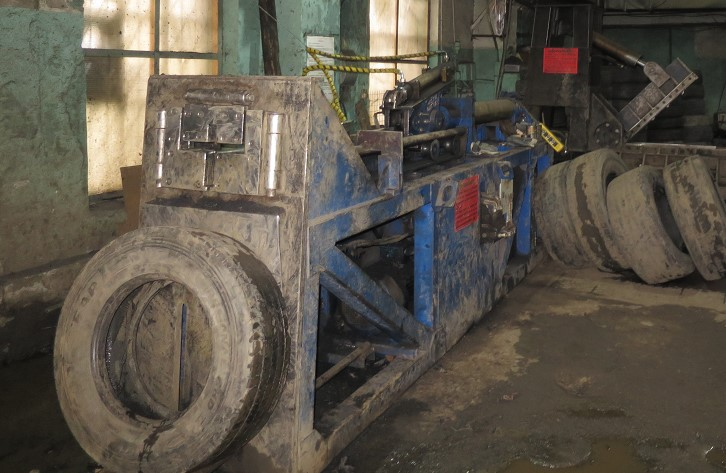
\includegraphics[angle=90,width=.49\textwidth]{1}
		\hfil \hfil%раздвигаем боксы по горизонтали
		\caption{}\label{fig:metka−1}}
	\parbox[t]{0.49\textwidth}{\centering
		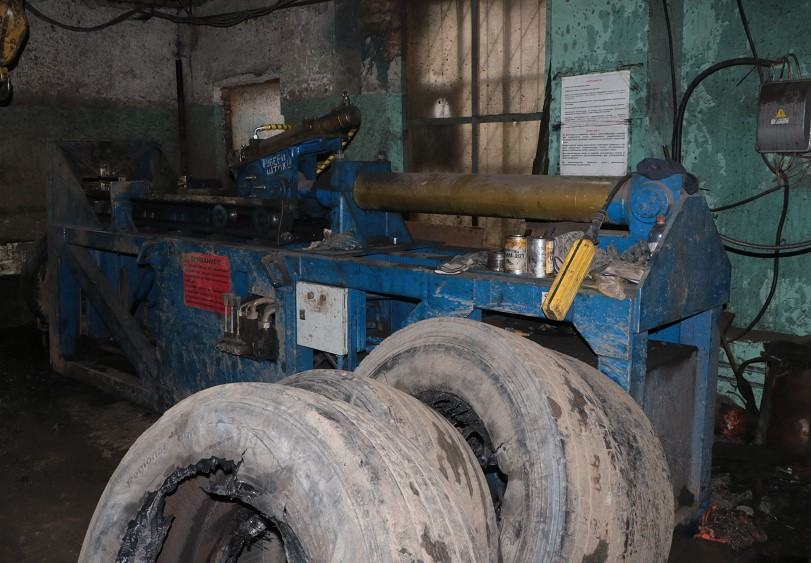
\includegraphics[angle=90,width=.49\textwidth]{2}
		\hfil \hfil%раздвигаем боксы по горизонтали
		\caption{}\label{fig:metka−2}}
\end{figure}


%\imgroot{160mm}{images/d1}{}{90}
%%\imgroot{160mm}{images/d2}{}{90} 
%\imgroot{160mm}{images/29}{}{90}
%\imgroot{160mm}{images/d2}{}{90}
%\imgroot{160mm}{images/21}{}{-90}
%\imgroot{160mm}{images/22}{}{-90}


%
%
%\begin{figure}[ht]\centering
%	\parbox[t]{0.49\textwidth}{\centering
%		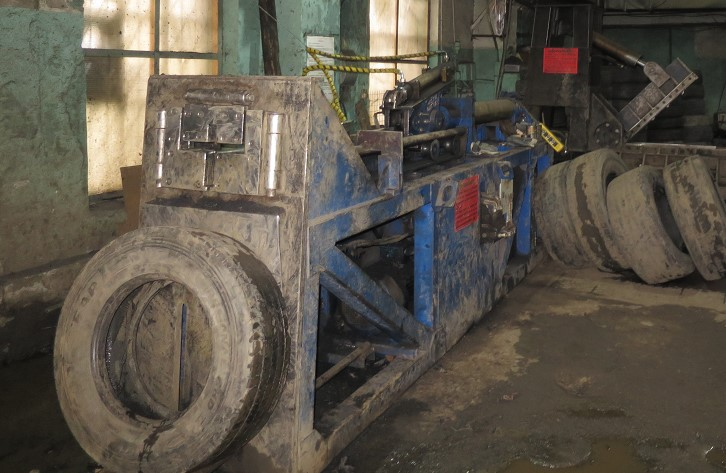
\includegraphics[width=.49\textwidth]{1}
%		\hfil \hfil%раздвигаем боксы по горизонтали
%		\caption{«подпись-1»}\label{fig:metka−1}}
%	\parbox[t]{0.49\textwidth}{\centering
%		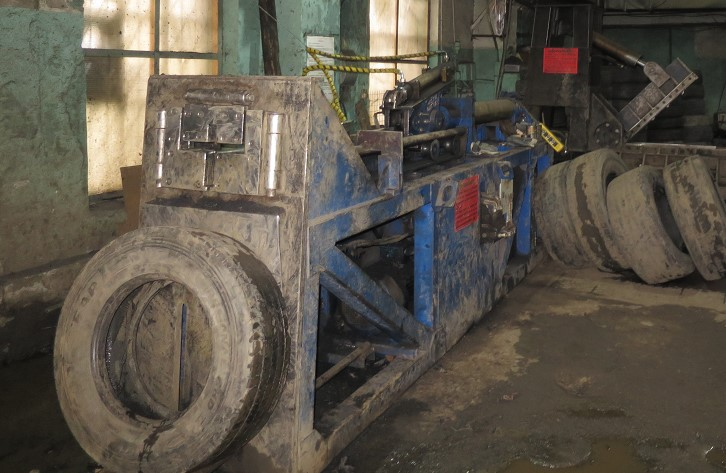
\includegraphics[width=.49\textwidth]{1}
%		\hfil \hfil%раздвигаем боксы по горизонтали
%		\caption{«подпись-1»}\label{fig:metka−1}}
%\end{figure}
%
%
%
%\begin{figure}[ht]\centering
%	\parbox[t]{0.49\textwidth}{\centering
%		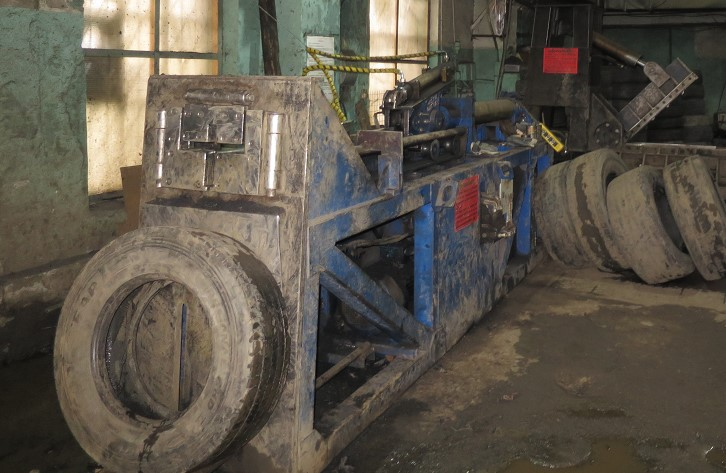
\includegraphics[width=.49\textwidth]{1}
%		\hfil \hfil%раздвигаем боксы по горизонтали
%		\caption{«подпись-1»}\label{fig:metka−1}}
%	\parbox[t]{0.49\textwidth}{\centering
%		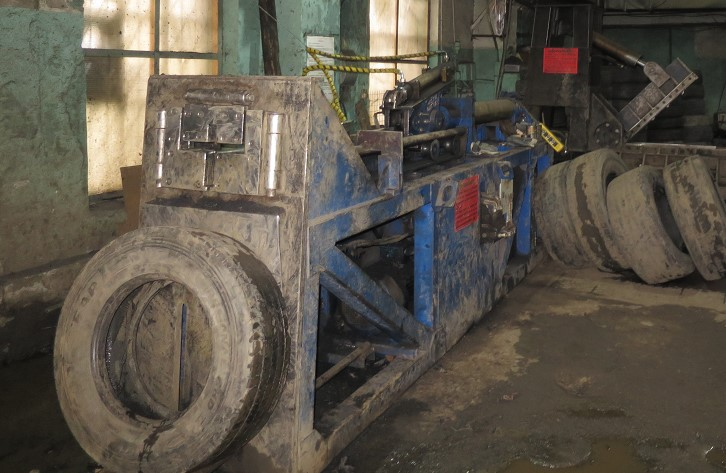
\includegraphics[width=.49\textwidth]{1}
%		\hfil \hfil%раздвигаем боксы по горизонтали
%		\caption{«подпись-1»}\label{fig:metka−1}}
%\end{figure}
%
%
%
%\begin{figure}[h]
%	\begin{minipage}[h]{0.47\linewidth}
%		\centering{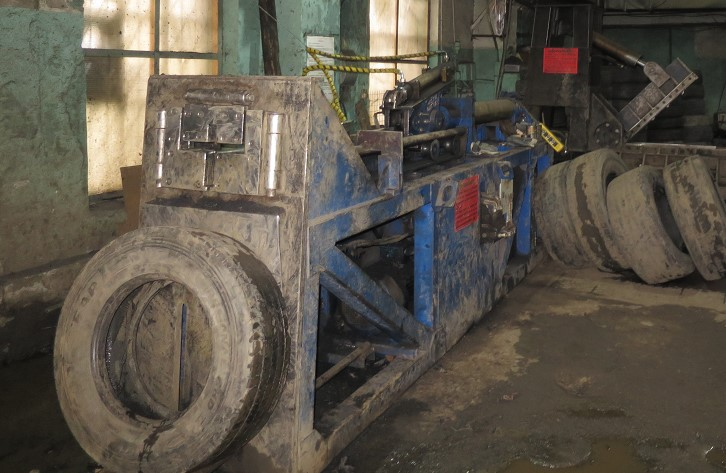
\includegraphics[width=1\linewidth]{1}} a) \\
%	\end{minipage}
%	\hfill
%	\begin{minipage}[h]{0.47\linewidth}
%		\centering{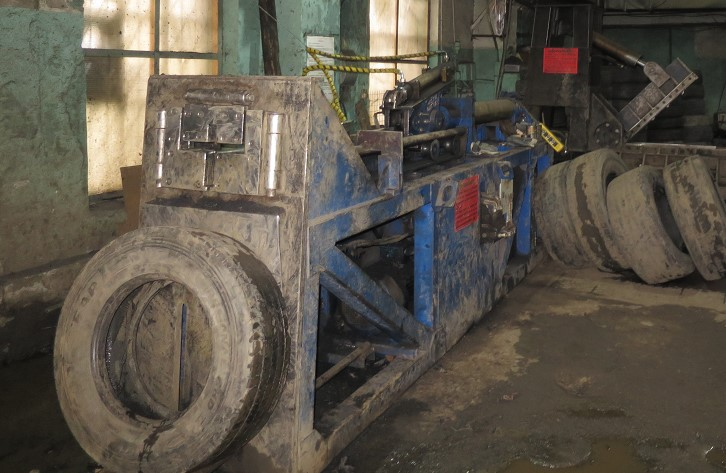
\includegraphics[width=1\linewidth]{1}} \\b)
%	\end{minipage}
%	\vfill
%	\begin{minipage}[h]{0.47\linewidth}
%		\centering{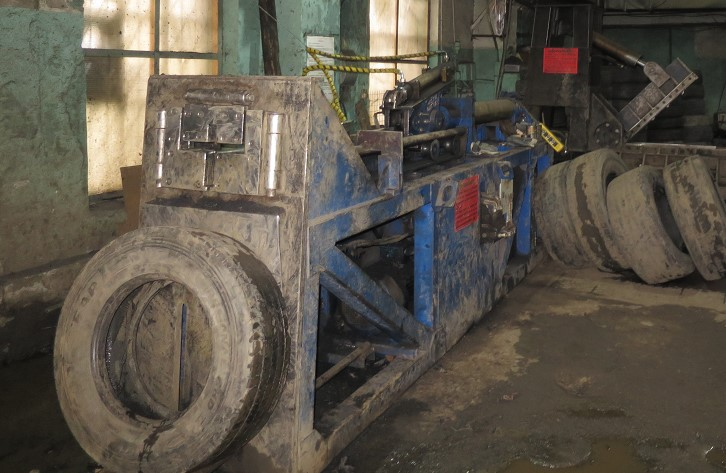
\includegraphics[width=1\linewidth]{1}} c) \\
%	\end{minipage}
%	\hfill
%	\begin{minipage}[h]{0.47\linewidth}
%		\centering{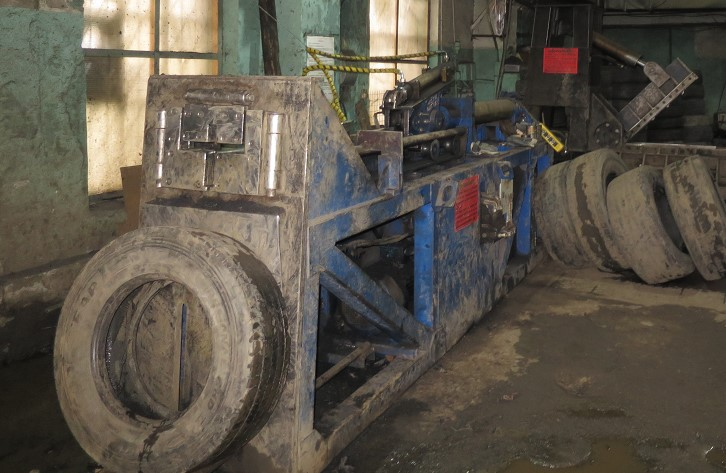
\includegraphics[width=1\linewidth]{1}} d) \\
%	\end{minipage}
%	\caption{Correlation signal peaks: a) numerical experiment, b)
%		registered correlation signals, c) intensity distribution of correlation
%		signals in numerical experiment, d) correlation signals intensity
%		distribution for DCRAW processed data.}
%	\label{ris:experimentalcorrelationsignals}
%\end{figure}
%
%
%
%\begin{figure}[ht!]  
%	\vspace{-4ex} \centering \subfigure[]{
%		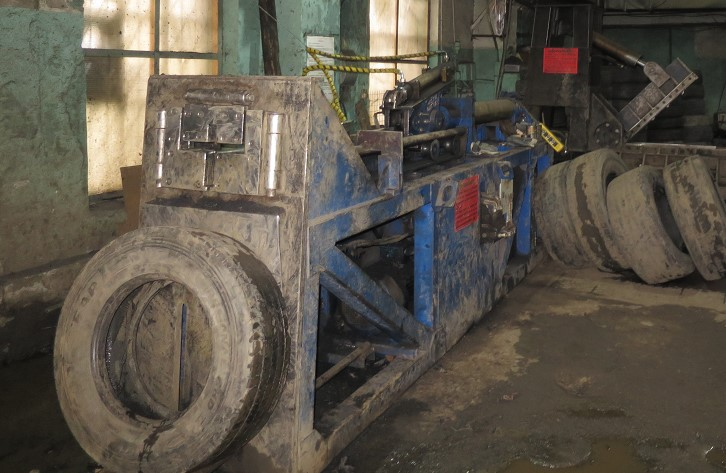
\includegraphics[width=0.25\linewidth]{1} \label{fig:actuatorscouplingSheme_decoupledcase} }  
%	\hspace{4ex}
%	\subfigure[]{
%		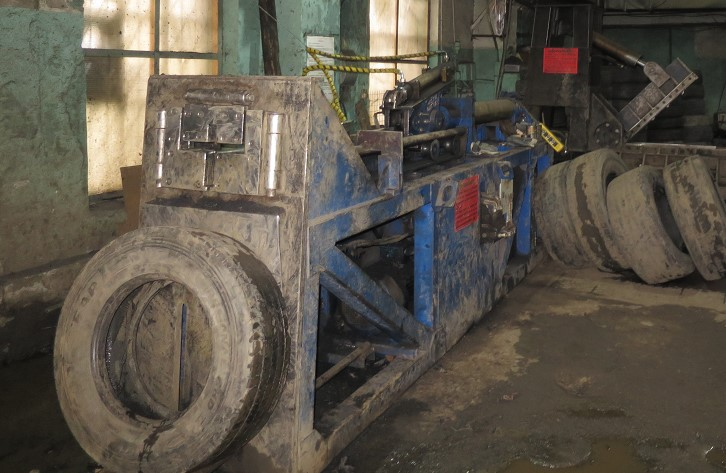
\includegraphics[width=0.25\linewidth]{1} \label{fig:actuatorscouplingSheme_nearestcoupledcase} }
%	\hspace{4ex}
%	\subfigure[]{ 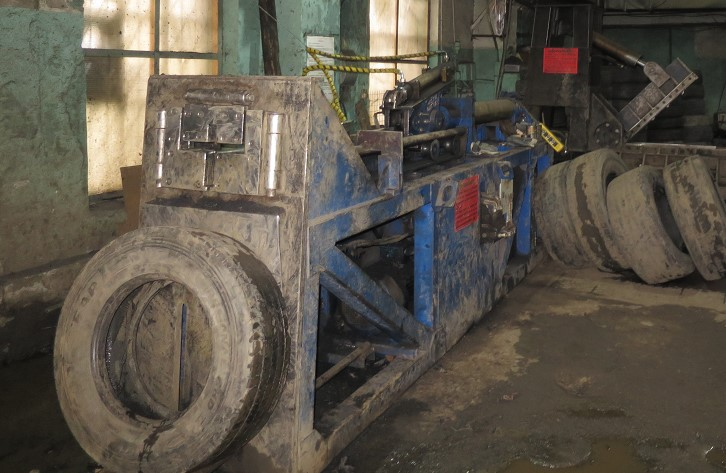
\includegraphics[width=0.24\linewidth]{1} \label{fig:actuatorscouplingSheme_nearestcoupled_and_diag_case} }  
%	\caption{Coupling cases for the DM models: \subref{fig:actuatorscouplingSheme_decoupledcase} decoupled case; \subref{fig:actuatorscouplingSheme_nearestcoupledcase} coupling between the closest neighbours; \subref{fig:actuatorscouplingSheme_nearestcoupled_and_diag_case} coupling between the closest neighbour and diagonally adjacent actuators.} \label{fig:threeDMcases}
%	\end{figure}
%
%\begin{figure}[ht!]  
%	\vspace{-4ex} \centering \subfigure[]{
%		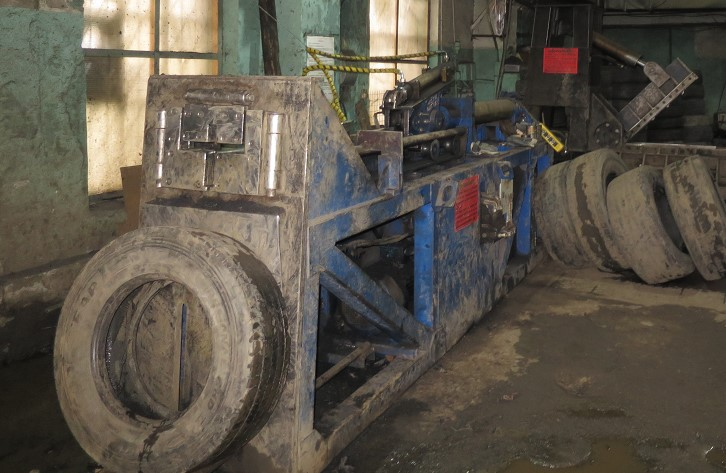
\includegraphics[width=0.25\linewidth]{1} \label{fig:actuatorscouplingSheme_decoupledcase} }  
%	\hspace{4ex}
%	\subfigure[]{
%		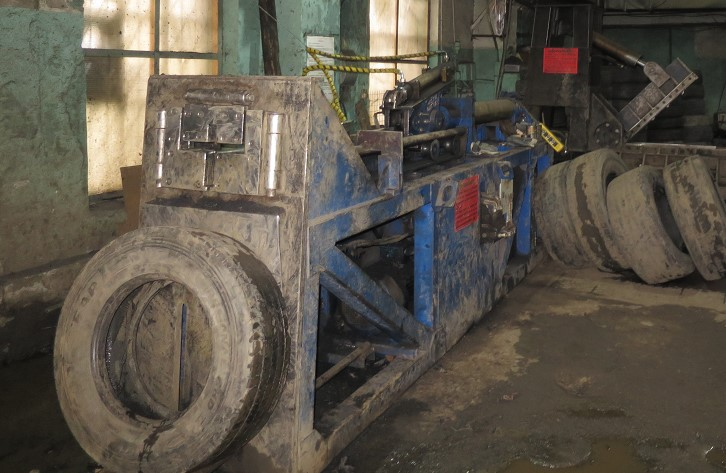
\includegraphics[width=0.25\linewidth]{1} \label{fig:actuatorscouplingSheme_nearestcoupledcase} }
%	\hspace{4ex}
%	\subfigure[]{ 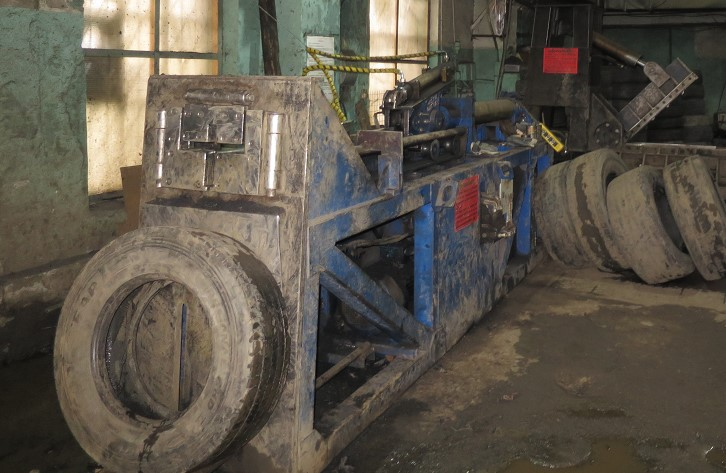
\includegraphics[width=0.24\linewidth]{1} \label{fig:actuatorscouplingSheme_nearestcoupled_and_diag_case} }  
%	\caption{Coupling cases for the DM models: \subref{fig:actuatorscouplingSheme_decoupledcase} decoupled case; \subref{fig:actuatorscouplingSheme_nearestcoupledcase} coupling between the closest neighbours; \subref{fig:actuatorscouplingSheme_nearestcoupled_and_diag_case} coupling between the closest neighbour and diagonally adjacent actuators.} \label{fig:threeDMcases}
%\end{figure}

\end{document}